\section{Background}\label{sec:background}

This section introduces the concepts the experiment builds on, for readers outside the LLM-systems niche.

\textbf{Self-hosting LLMs.} Open-weight models (\eg the Qwen, Llama, Gemma, and Granite families) can be downloaded and served on hardware the user controls, instead of being consumed through a provider's API. Self-hosting trades the convenience and raw capability of frontier APIs for privacy (data never leaves the machine), cost predictability, reproducibility (pinned weights, no silent model updates), and independence. Its practical viability depends on whether a locally-served model is accurate \emph{enough} and cheap \emph{enough} on the user's actual workload, in energy as well as in money.

\textbf{Dense vs.\ Mixture-of-Experts architectures.} In a \emph{dense} transformer, every parameter participates in every token's computation, so inference cost grows with total model size. A \emph{Mixture-of-Experts} (MoE) model replaces feed-forward blocks with many parallel ``experts'' of which a router activates only a few per token: \texttt{Qwen3-30B-A3B} holds 30.5B parameters but activates only $\sim$3B per token. MoE thus promises large-model quality at small-model per-token compute, an attractive proposition for self-hosting, where the energy budget is the user's own. Whether the promise holds on a real agentic workload, where proposal \emph{quality} feeds back into downstream compute, is this experiment's architectural question.

\textbf{Quantization and intra-model configuration.} Model weights are typically released at 16-bit precision; \emph{quantization} compresses them to lower precision (here int4, $\sim$4 bits per weight), shrinking memory and energy per token at some accuracy risk. Quantization level, sampling temperature, context handling, and serving-stack settings together form the model's \emph{intra-model configuration}. In this experiment the intra-model configuration is deliberately \emph{fixed} (AWQ int4, temperature 0.7, reasoning disabled) so that Stage~1 isolates the architectural effect; varying these settings for further optimization is Stage~2 of the staged design (Section~\ref{sec:planning}).

\textbf{Agentic loops and \texttt{autoresearch}.} An \emph{agentic} workload invokes an LLM repeatedly inside a feedback loop rather than once per user prompt. Karpathy's \texttt{autoresearch} \cite{karpathy2026autoresearch} is an agentic AutoML system whose iteration cycle is shown in Figure~\ref{fig:autoresearch-loop}. Each iteration starts from \texttt{program.md}, a Markdown file holding the task description, the current training recipe of the inner workload, and the history of past attempts. The LLM \emph{proposer} reads this state and proposes a \emph{mutation}: a concrete diff to the recipe (\eg a hyperparameter change, an architectural tweak, a data-pipeline edit). The mutated recipe is trained for a bounded, fixed-time experiment. In this study the inner workload is a compact convolutional network on CIFAR-10; \texttt{autoresearch}'s default inner workload is \texttt{nanochat}, a small LLM training pipeline, and the swap (motivated by the schedule, Section~\ref{sec:execution}) preserves the protocol's semantics. The resulting checkpoint is scored by validation accuracy (\texttt{val\_acc}) on a held-out split. A mutation becomes the new best only when \texttt{val\_acc} exceeds the previous best by more than the measured threshold $\epsilon$. A below-threshold mutation is retained \emph{provisionally} as context for the next proposal; a later new best absorbs that chain, whereas reaching the configured \emph{patience} rolls the whole provisional chain back to the best recipe. The loop repeats until the session's \emph{loop budget} (maximum number of outer-loop attempts) is exhausted; internal proposer retries stay within one attempt. Guard rejection, proposer error, and training error consume attempts and are logged without becoming retained mutations. At exhaustion, any pending provisional chain is rolled back and the best checkpoint is evaluated once on the CIFAR-10 test set. Each attempt records its outcome and available token and timing metadata in the session log that this experiment parses for its dependent variables. A session therefore interleaves many LLM inferences with many short, fixed-length GPU training runs, and total energy depends jointly on the proposer and on the loop's configuration; this is why both appear as factors in this study. Validation accuracy and test-set accuracy serve as the ground-truth accuracy metrics.

\begin{figure}[htbp]
\centering
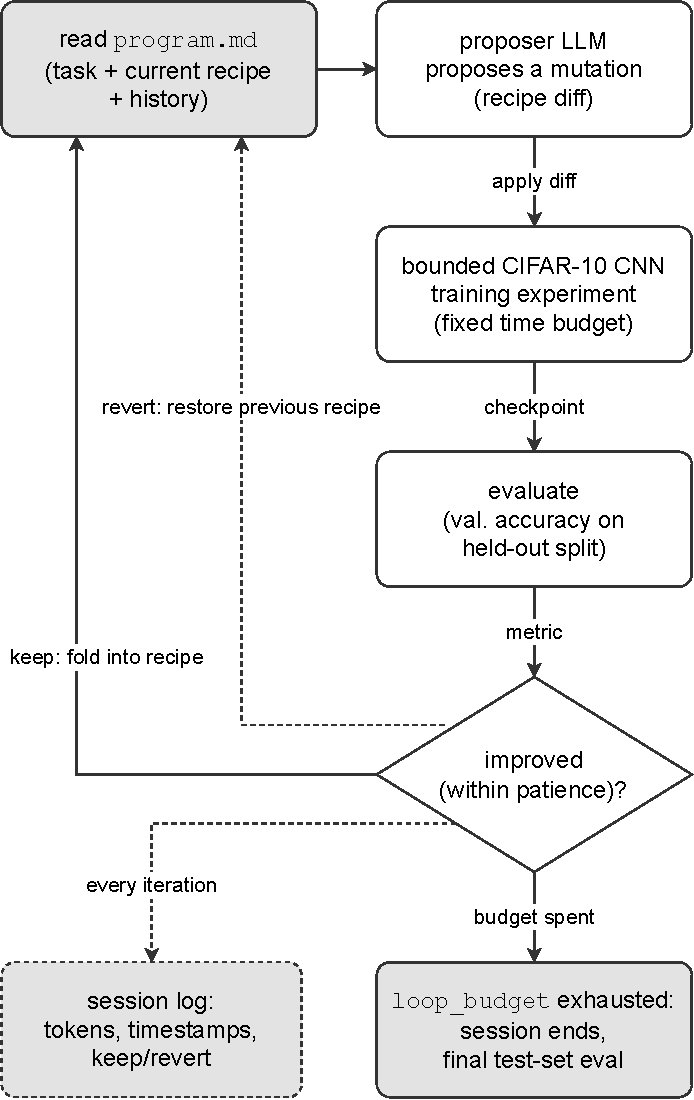
\includegraphics[width=\columnwidth]{figures/autoresearch_loop.drawio.pdf}
\caption{The implemented \texttt{autoresearch} loop. Every scheduled outer-loop attempt consumes
the fixed loop budget, including proposer error, guard rejection, and training error. A valid
candidate is kept only when \texttt{val\_acc} exceeds the best score by more than
$\epsilon$; otherwise a valid below-threshold candidate remains provisional until a later keep absorbs the chain,
or patience or budget exhaustion rolls it back. At budget exhaustion, the best
checkpoint is evaluated once on the test split.}
\Description{Flowchart showing mutation proposal, proposer and guard failures, bounded training, training error, epsilon-qualified keep, provisional retention, patience rollback, fixed-budget accounting, and final rollback plus one test evaluation.}
\label{fig:autoresearch-loop}
\end{figure}

\textbf{Energy measurement.} Modern hardware exposes energy and power counters. NVIDIA's NVML \cite{nvidia2026nvml} reports board power per GPU; the AMD host used here exposes a CPU-package energy counter through \texttt{EnergiBridge} \cite{sallou2023energibridge}. The archived trace does not contain a separate DRAM counter. Integrating or differencing these counters over the same timestamp bounds yields energy for the measured components in joules, but not wall-power or full-system energy. Because NVML is per-GPU, placing training and proposing on separate devices provides a useful device-associated decomposition, while still including each device's idle and weight-residency draw. The \texttt{experiment-runner} framework \cite{karsten2025experimentrunner} automates the surrounding protocol: run tables, factor randomization, instrumentation lifecycle, and result collection.
